\documentclass{labo}

\usepackage{charter}
\usepackage[utf8x]{inputenc}
\usepackage[T1]{fontenc}
\usepackage{ucs}
\usepackage{amsthm} %numéroter les questions
% \usepackage[frenchb]{babel}
\usepackage{datetime}
\usepackage{xspace} % typographie IN
\usepackage{hyperref}% hyperliens
\usepackage[all]{hypcap} %lien pointe en haut des figures
\usepackage[french]{varioref} %voir x p y
\usepackage{fancyhdr}% en têtes
\usepackage[]{graphicx} %include pictures
% \usepackage{pgfplots}
\usepackage[americanresistors,siunitx]{circuitikz}
\usepackage[]{gnuplottex}
\usepackage{ifthen}
\usepackage{mathastext} % math as standfard text : units are respecting typography conventions.
\usepackage[]{subfig}
\usepackage[]{attachfile}
\usepackage{tikz}
\usetikzlibrary{babel,positioning,calc}
\usepackage{siunitx}
\usepackage{amssymb}
\usepackage{xcolor}
\usepackage{float}
\usepackage[normalem]{ulem}
\usepackage{todonotes}

\usepackage{framed}

%%%%%%%%%%%%
% Tables
%%%%%%%%%%%%
\usepackage{booktabs}
\renewcommand{\arraystretch}{1.1} % Opens up the table a tad
\usepackage{multicol}
\usepackage{multirow}

\newboolean{koriG}
\ifx\koriG\undefined
\correction{false}
\else
\correction{true}
\fi

\newcommand{\itgv}[1]{\ifthenelse{\boolean{corrige}}{{\color{blue}#1}}{}} %si corrigé vrai...
\newcommand{\ifgv}[1]{\ifthenelse{\boolean{corrige}}{}{#1}} %si corrigé vrai...

% \correction{false}
%\correction{true}

\definecolor{darkblue}{rgb}{0,0,0.5}

%% fancy header & foot
\pagestyle{fancy}
\lhead{[EOSI40] Instrumentation labs\\ Lab 3: Rigol DG1022 Signal Generator command}
\rhead{v0.9.0 \\ page \thepage}
\chead{\ifthenelse{\boolean{corrige}}{Corrigé}{}}
\cfoot{}
%%

\author{GEI}


\setlength{\parindent}{0pt}


%from SO: kinky cross for wires
\tikzset{
  declare function={% in case of CVS which switches the arguments of atan2
    atan3(\a,\b)=ifthenelse(atan2(0,1)==90, atan2(\a,\b), atan2(\b,\a));},
  kinky cross radius/.initial=+.125cm,
  @kinky cross/.initial=+, kinky crosses/.is choice,
  kinky crosses/left/.style={@kinky cross=-},kinky crosses/right/.style={@kinky cross=+},
  kinky cross/.style args={(#1)--(#2)}{
    to path={
      let \p{@kc@}=($(\tikztotarget)-(\tikztostart)$),
          \n{@kc@}={atan3(\p{@kc@})+180} in
      -- ($(intersection of \tikztostart--{\tikztotarget} and #1--#2)!%
             \pgfkeysvalueof{/tikz/kinky cross radius}!(\tikztostart)$)
      arc [ radius     =\pgfkeysvalueof{/tikz/kinky cross radius},
            start angle=\n{@kc@},
            delta angle=\pgfkeysvalueof{/tikz/@kinky cross}180 ]
      -- (\tikztotarget)}}}


\begin{document}
\tptitle{}{Lab 3: Rigol DG1022 Signal Generator command}

The objective of this lab is to use SCPI commands to control the signal generator Rigol DG1022.
A command is a particular character string, specifying a command and arguments.
Rigol, the device manufacturer, has a detailed documentation about the command syntax that can be used with the DG1000 family.


To actually use those commands, you will need to handle VIs associated to the character strings.
The commands are then transmitted using the VISA protocol.
Figure~\ref{fig:VISA} shows those blocks in the control palette.
The first step is to open a communication, then there must be a delay of 150ms between eaach command.
Finally, the communication must be closed.

To handle character strings, two particularly useful blocks are the ``multiline strings'' to allow the user to choose between several options through the front panel.

% INSERT FIGURE control palette

An other block can convert digital data into character strings for the user interface, using the following convention:
\begin{itemize}
  \item Specify a character for the decimal separator
  \item Send a string linked to the command
  \item A space
  \item Format the number into fract/sci
\end{itemize}

\begin{framed}
  Proof check this whole part, it makes no sense.
\end{framed}



\section{Activation interface for the Rigol generator}
Install the drivers for the device first.
\begin{framed}
Include the content of the appendix here directly.
\end{framed}

Build an interface that allows the user to enable or disable the channels of the generator.
Figure~\ref{fig:block-diagram-channel} exploits event and boolean structures to do so, may it inspire you to add a second channel.

\begin{figure}[ht!]
\centering
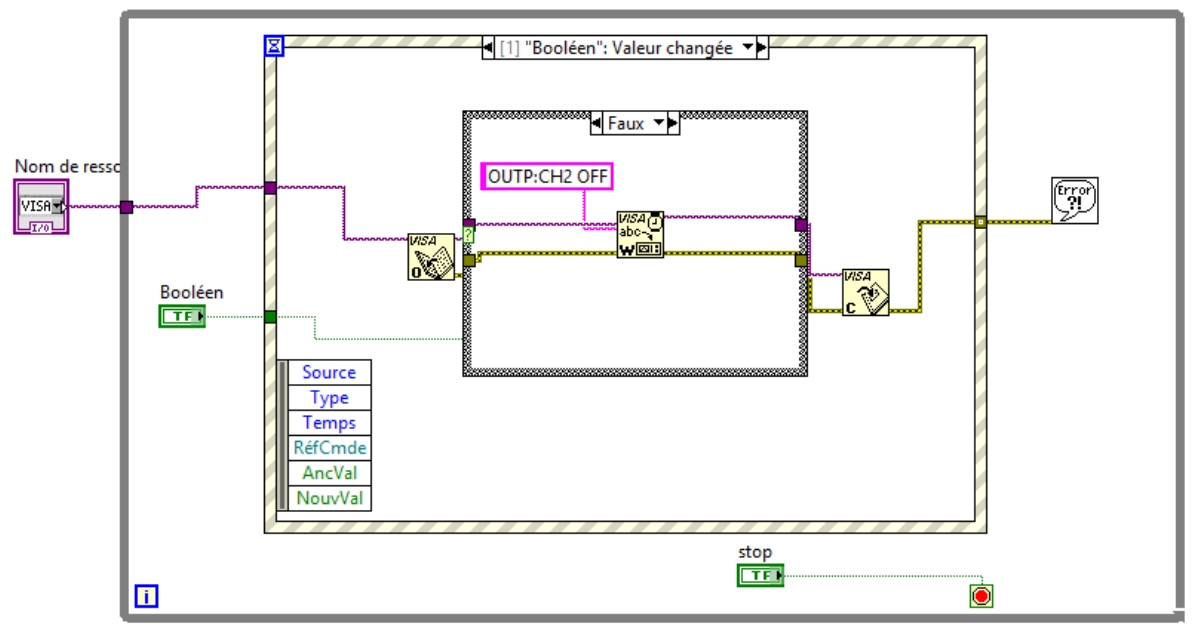
\includegraphics[width=\linewidth]{block-diagram-channel.png}
\caption{Block diagram of a program controlling a single channel of the signal generator.}
\label{fig:block-diagram-channel}
\end{figure}


\section{Rigol DG1022 Interface -- The Remake}
Build an interface that allows to configure the Rigol generator settings, similar to Figure~\ref{fig:front-panel-Rigol}:
\begin{itemize}
  \item Waveform function
  \item Amplitude
  \item Peak-to-peak voltage
  \item DC offset
  \item Frequency
  \item Duty cycle in case of a square signal
\end{itemize}
A ``configure'' button should allow the user to update the configuration.
The buttons to control the channels activation should also be reused.

Implement one feature at a time and remember that you can nest your VIs.

\begin{figure}[ht!]
\centering
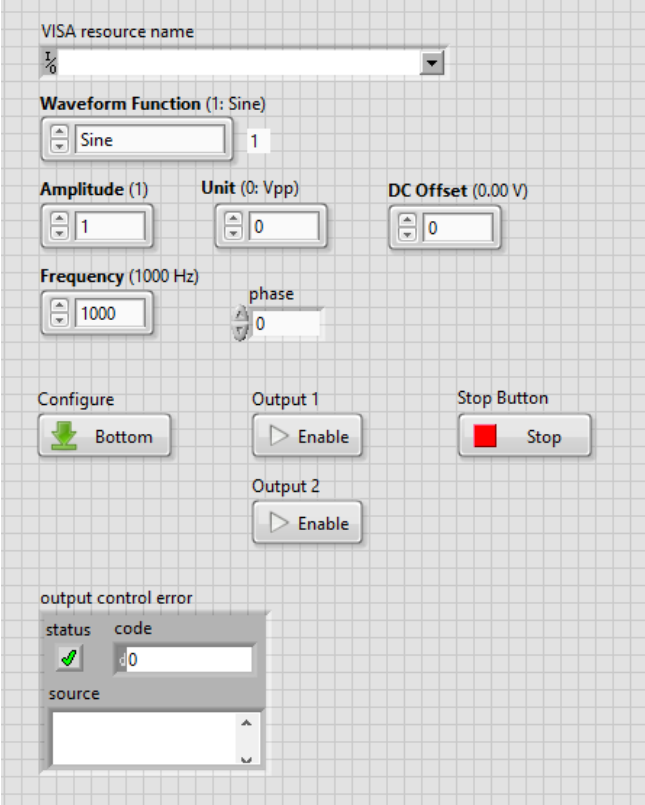
\includegraphics[width=.5\linewidth]{front-panel-Rigol.png}
\caption{}
\label{fig:front-panel-Rigol}
\end{figure}



\section{Oscilloscope interface}



\section{Interconnect both devices}



\section{Bonus: Validation testing}
Validate your configuration of the generator by reading the device registers and display the result of this validation.






% \begin{figure}[ht!]
% \centering
% 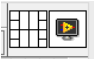
\includegraphics[]{mod-icon-conn.png}
% \caption{}\label{fig:mod-icon-conn}
% \end{figure}



% \Question{}{}
\end{document}
